\chapter{Описание процедур измерения}
\label{sec:measurement}
Упрощенная схема порта Ввода/Вывода ATmega показана  на рисунке ~\ref{fig:port}.
Ключ PUD отключает все подтягивающие резисторы ATmega. Состояние выхода порта может быть переключено ключом DD. 
Вход порта может управляться независимо от ключа DD. Ключ PORT обычно определяет выходной уровень, но также и 
переключает подтягивающий резистор. Поскольку ключи PORT и DD не могут быть изменены одновременно, а только один 
за другим, подтягивающие резисторы могут нарушить измерение. Поэтому я предварительно отключаю подтягивающие 
резисторы ключом PUD. Конечно, все ключи - электронные и величины сопротивлений резисторов \(19~\Omega\) 
и \(22~\Omega\) приблизительны.

\begin{figure}[H]
\centering
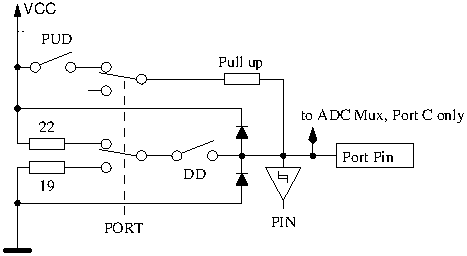
\includegraphics[width=.8\textwidth]{../FIG/port.pdf}
\caption{Упрощенная схема каждого вывода порта ATmega}
\label{fig:port}
\end{figure}

Каждый  из трех измерительных щупов Тестера конструктивно соединен с тремя выводами портов ATmega, которые показаны 
на упрощенной схеме испытательного вывода TP2 (средний, из трех выводов TP, TP2 и TP3) на рисунке~\ref{fig:terminal}.

\begin{figure}[H]
\centering
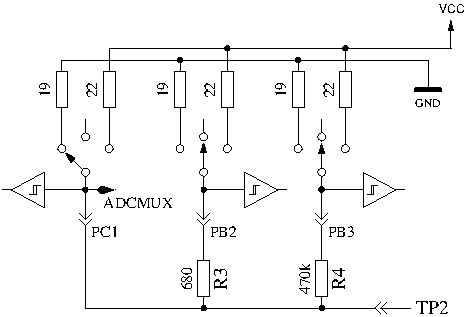
\includegraphics[width=.8\textwidth]{../FIG/terminal.pdf}
\caption{Упрощенная схема каждого испытательного вывода щупа TP}
\label{fig:terminal}
\end{figure}

Каждый испытательный вывод (измерительный порт, щуп) может использоваться в качестве цифрового или аналогового 
входа. Эта возможность измерения не зависит от использования порта в качестве выхода. Каждый испытательный порт 
может быть переключен на вывод. В этом состоянии он может быть подключен к GND (\(0~V\)) или VCC (\(+5~V\)) 
непосредственно или через резистор \(680~\Omega\) или резистор \(470~k\Omega\).
Таблица~\ref{tab:case} показывает все возможные комбинации измерений. Заметьте, что положительное состояние может 
быть получено подключением непосредственно к VCC (порт C) или через резистор \(680~\Omega\) к VCC (Порт B). Такая 
же возможность есть и для отрицательного состояния при подключении испытательного порта к GND. Состояние 
испытательного щупа может быть открытым (Вход), соединённым через резистор \(470~k\Omega\) к VCC или GND, 
или испытательный щуп может быть подключен через резистор \(680~\Omega\) к VCC или GND.

\begin{table}[H]
  \begin{center}
    \begin{tabular}{| l | c | c | c |}
    \hline
      & Состояние щупа 1 & Состояние щупа 2 & Состояние щупа 3 \\
    \hline
   1. & положительное    &  отрицательное    &  тест \\
   2. & положительное    &  тест       & отрицательное \\
   3. & тест        &  отрицательное    & положительное \\
   4. & тест        &  положительное    & отрицательное \\
   5. & отрицательное     &  тест       & положительное \\
   6. & отрицательное     &  положительное    &  тест  \\
    \hline
    \end{tabular}
  \end{center}
  \caption{Все комбинации измерений}
  \label{tab:case} 
\end{table}

Если Тестер сконфигурирован для измерения ёмкости, то Тестер попытается разрядить конденсаторы, 
соединённые со всеми испытательными выводами. Если разрядка потерпит неудачу, которая означает,
что остаточное напряжение высокое, разрядка будет прервана приблизительно через 12 секунд
с выводом сообщения \inquotes{Cell!}. Это может произойти так же, если никакой конденсатор не связан ни с каким 
испытательным выводом. 
Причиной может быть то, что напряжения отключения выбрано низким для этого ATmega. Вы можете выбрать более 
высокое напряжение опцией CAP\_EMPTY\_LEVEL в Makefile.
